

\begin{frame}{Polyhedra}


\begin{definition}
  A polyhedron $P\subseteq\setR^n$ is a set of the form $P = \{ x \in
   \setR^n \colon Ax\leq b\}$ for some $A\in \setR^{m\times n}$ and
  some $b \in \setR^m$.
\end{definition}

\begin{columns}
    \begin{column}{.5\textwidth}     
    \begin{displaymath}
      A =
      \begin{pmatrix}
        3 & 6 \\
        8 & 4 \\
        1 & 0 \\
        0 & 1 \\
        -1 & 0 \\
        0 & -1
      \end{pmatrix},
    \quad b = 
      \begin{pmatrix}
        30 \\ 44 \\ 5 \\ 4 \\ 0 \\ 0
      \end{pmatrix}:
    \end{displaymath}
 
    \end{column}
    \begin{column}{.5\textwidth}
      
      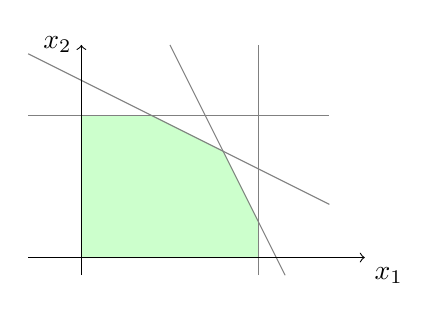
\begin{tikzpicture}[scale=.45]       
     
      \filldraw[fill=green!20,draw=green!20!](0,0) -- (0,4) -- (2,4) --
      (4,3) -- (5,1) -- (5,0) -- (0,0); 
      
      
      \draw [-,draw=gray] (7,1.5) -- (-1.5,5.75) ;
      \draw [-,draw=gray] (-1.5,4) -- (7,4) ;
      \draw [-,draw=gray] (5,-.5) -- (5,6) ;
      \draw [-,draw=gray] (2.5,6) -- (5.75,-.5) ;
      
      
          
      \draw[->] (-1.5,0) -- (8,0) node[below right] {$x_1$}; \draw[->]
      (0,-.5) -- (0,6) node[left] {$x_2$};
      
%      \draw[draw=blue] (-1.50000000000000,
%      7.40000000000000)node[left]{\small  
%        \color{blue}{$  \beta = 775$}} --
%      (8.37500000000000, -0.500000000000000) ; 
      
%      \filldraw [red] (4,3) circle (3pt)node[above right] {$(4,3)$};
      
          
%      \foreach \x in {1,...,7}
 %     \draw (\x cm,1pt) -- (\x cm,-1pt) node[anchor=north] {$\x$};
 %     \foreach \y in {1,...,5}
 %     \draw (1pt,\y cm) -- (-1pt,\y cm) node[anchor=east] {$\y$};     
    \end{tikzpicture} 


    \end{column}       
  \end{columns}

\end{frame}







\begin{frame}{Convex sets}


\begin{definition}
  \label{conv:def:2}
  A set $K\subseteq\setR^n$ is \emph{convex} if for each $u,v \in K$
  and $\lambda \in [0,1]$ the point $\lambda u+(1-\lambda)v$ is also
  contained in $K$. \end{definition}

\bigskip 
\centering
  
\includegraphics[height=3cm]{../figures/exconv.pdf} 



  
  \begin{columns}
    \begin{column}{.5\textwidth}
      
    \end{column}
    \begin{column}{.5\textwidth}
      
    \end{column}       
  \end{columns}
\end{frame}






\begin{frame}{Halfspaces}

  \begin{definition}    
    A \emph{halfspace} is a set  of the form
    \begin{displaymath}
  \{ x \in \R^n \colon a^Tx \leq \beta\}. 
\end{displaymath}

A \emph{hyperplane} is a set of the form 
\begin{displaymath}
  \{ x \in \R^n \colon a^Tx = \beta\}. 
\end{displaymath} 

  \end{definition}

  
  \begin{columns}
    \begin{column}{.5\textwidth}
      
    \end{column}
    \begin{column}{.5\textwidth}
      
    \end{column}       
  \end{columns}
\end{frame}





\begin{frame}{Halfspaces are convex}
\begin{lemma}
    A half-space is convex. 
  \end{lemma}
  \begin{columns}
    \begin{column}{.5\textwidth}
      
    \end{column}
    \begin{column}{.5\textwidth}
      
    \end{column}       
  \end{columns}
\end{frame}



\begin{frame}{}

  \begin{columns}
    \begin{column}{.5\textwidth}
      
    \end{column}
    \begin{column}{.5\textwidth}
      
    \end{column}       
  \end{columns}
\end{frame}




\begin{frame}{Intersections of convex sets}
\begin{lemma}
  \label{lem:1}
  Let $I$ be an index set and $C_i \subseteq \R^n$ be convex sets for
  each $i \in I$, then $\cap_{i \in I}C_i$ is a convex set.
\end{lemma}

\begin{corollary}
  A polyhedron is a convex set.  
\end{corollary}


\end{frame}





\begin{frame}{}

  \begin{columns}
    \begin{column}{.5\textwidth}
      
    \end{column}
    \begin{column}{.5\textwidth}
      
    \end{column}       
  \end{columns}
\end{frame}




\begin{frame}{Valid inequalities}


 



  \begin{columns}
    \begin{column}{.5\textwidth}
       \begin{definition}
    $a^Tx \leq \beta$ is \emph{valid} for $K \subseteq \R^n$ if for each $x^* \in K$:   $$a^Tx^* \leq \beta$$


    If in addition $(a^Tx = β) \cap K \neq\emptyset$, then
    $a^Tx\leq β$ is a \emph{supporting inequality} and $a^Tx = β$ is a
    \emph{supporting hyperplane}
\end{definition}

    \end{column}
    \begin{column}{.5\textwidth}
      
    \end{column}       
  \end{columns}
\end{frame}




\begin{frame}{Extreme points }



  
  
  \begin{columns}
    \begin{column}{.5\textwidth}
      \begin{definition}
  Let $K \subseteq \R^n$ be  convex. $x^* \in K$ is
 \emph{extreme point} or \emph{vertex} of $K$ if there exists a valid inequality $a^Tx \leq \beta$ of $K$ such that 
 \begin{displaymath}
   \{x^*\} = K \cap \{x \in \R^n \colon a^Tx = \beta\}.  
 \end{displaymath}
\end{definition}

    \end{column}
    \begin{column}{.5\textwidth}
      \centering
  
\includegraphics[height=3cm]{../figures/ExtremePoint.pdf} 



    \end{column}       
  \end{columns}
\end{frame}



\begin{frame}{Vertices of polyhedra -- algebraic characterization}

\begin{theorem}
  \label{thr:1}
  Let $P = \{x \in \R^n \colon Ax \leq b\}$ be a polyhedron. $x^* ∈ P$ is  extreme point iff  there is  sub-system $A'x \leq b'$ of  $Ax \leq b$  s.t. 
  \begin{enumerate}[i)]
  \item $x^*$ satisfies all inequalities of $A'x \leq b'$ with
    equality. \label{item:1}
  \item $A'$ has $n$ rows and $A'$ is non-singular. \label{item:2}
  \end{enumerate}  
\end{theorem}
{\small 
\begin{columns}
    \begin{column}{.5\textwidth}     
    \begin{displaymath}
      A =
      \begin{pmatrix}
        3 & 6 \\
        8 & 4 \\
        1 & 0 \\
        0 & 1 \\
        -1 & 0 \\
        0 & -1
      \end{pmatrix},
    \quad b = 
      \begin{pmatrix}
        30 \\ 44 \\ 5 \\ 4 \\ 0 \\ 0
      \end{pmatrix}:
    \end{displaymath}
 
    \end{column}
    \begin{column}{.5\textwidth}
      
      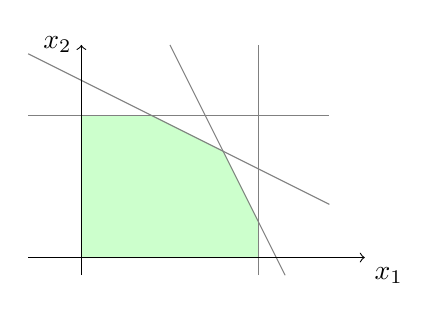
\begin{tikzpicture}[scale=.45]       
     
      \filldraw[fill=green!20,draw=green!20!](0,0) -- (0,4) -- (2,4) --
      (4,3) -- (5,1) -- (5,0) -- (0,0); 
      
      
      \draw [-,draw=gray] (7,1.5) -- (-1.5,5.75) ;
      \draw [-,draw=gray] (-1.5,4) -- (7,4) ;
      \draw [-,draw=gray] (5,-.5) -- (5,6) ;
      \draw [-,draw=gray] (2.5,6) -- (5.75,-.5) ;
      
      
          
      \draw[->] (-1.5,0) -- (8,0) node[below right] {$x_1$}; \draw[->]
      (0,-.5) -- (0,6) node[left] {$x_2$};
      
%      \draw[draw=blue] (-1.50000000000000,
%      7.40000000000000)node[left]{\small  
%        \color{blue}{$  \beta = 775$}} --
%      (8.37500000000000, -0.500000000000000) ; 
      
%      \filldraw [red] (4,3) circle (3pt)node[above right] {$(4,3)$};
      
          
%      \foreach \x in {1,...,7}
 %     \draw (\x cm,1pt) -- (\x cm,-1pt) node[anchor=north] {$\x$};
 %     \foreach \y in {1,...,5}
 %     \draw (1pt,\y cm) -- (-1pt,\y cm) node[anchor=east] {$\y$};     
    \end{tikzpicture} 


    \end{column}       
  \end{columns}}



  
  \begin{columns}
    \begin{column}{.5\textwidth}
      
    \end{column}
    \begin{column}{.5\textwidth}
      
    \end{column}       
  \end{columns}
\end{frame}








\begin{frame}{Optimal solutions and vertices}


\begin{theorem}
  \label{thr:2}
  If a linear program $\max\{c^Tx \colon x \in \R^n, \, Ax \leq b\}$
  is feasible and bounded and if $\rank(A) = n$, then the linear program has an optimal solution that is  an extreme point. 
\end{theorem}


  
  \begin{columns}
    \begin{column}{.5\textwidth}
      
    \end{column}
    \begin{column}{.5\textwidth}
      
    \end{column}       
  \end{columns}
\end{frame}







\begin{frame}{}

  \begin{columns}
    \begin{column}{.5\textwidth}
      
    \end{column}
    \begin{column}{.5\textwidth}
      
    \end{column}       
  \end{columns}
\end{frame}






\begin{frame}{Bounded LP has optimal solution}



\begin{corollary}
  \label{co:12}
  A linear program $\max \{ c^Tx : x ∈ ℝ^n, \, Ax ≤ b\}$ which is feasible and bounded has an optimal solution. 
\end{corollary}

  
  \begin{columns}
    \begin{column}{.5\textwidth}
      
    \end{column}
    \begin{column}{.5\textwidth}
      
    \end{column}       
  \end{columns}
\end{frame}






\begin{frame}{A first (inefficient) algorithm}

  Given $\max\{c^T x : x ∈ ℝ^n, \, Ax ≤b \}$  w.l.o.g. $\rank(A) =n$
  
  \begin{itemize}
  \item  Initialize $M = ∅$ 
  \item Enumerate all sets of $n$ row-vectors that are basis of $ℝ^n$
    \begin{itemize}
    \item    Solve $A'x = b'$ for corresponding system
    \item If for solution $x^*$: $Ax^* ≤ b$ then $M = M + x^*$      
    \end{itemize}
  \item Output point of  $M$  with largest objective function value 
  \end{itemize}

  \bigskip

  \begin{theorem}
    If LP is bounded then algorithm above computes optimal solution. 
  \end{theorem}


  \begin{alertblock}{We will see ...}
    ... we can do much better. 
  \end{alertblock}
\end{frame}





\begin{frame}{Bounded continuous functions}

\begin{theorem}

  Let $X\subseteq\setR^n$ be compact and $f: X \to \setR$ be continuous. Then $f$ is
  bounded and there exist
  points $x_1,x_2 \in X$ with $f(x_1) = \sup\{ f(x) \colon  x \in X\}$ and
  $f(x_2) = \inf \{ f(x) \colon x \in X\}$. 
\end{theorem}
  
  \begin{columns}
    \begin{column}{.5\textwidth}
      
    \end{column}
    \begin{column}{.5\textwidth}
      
    \end{column}       
  \end{columns}
\end{frame}







\begin{frame}{Separation theorem}

\begin{theorem}

  Let $K\subseteq\setR^n$ be a closed  convex set and $x^* \in \setR^n \setminus K$, then there
  exists an inequality $a^Tx ≤ \beta$ such that $a^T y < \beta$ holds for all
  $y \in K$ and $a^Tx^*>\beta$. 
\end{theorem}

  \begin{columns}
    \begin{column}{.5\textwidth}
      
    \end{column}
    \begin{column}{.5\textwidth}
      
    \end{column}       
  \end{columns}
\end{frame}






\begin{frame}{}

  \begin{columns}
    \begin{column}{.5\textwidth}
      
    \end{column}
    \begin{column}{.5\textwidth}
      
    \end{column}       
  \end{columns}
\end{frame}






\begin{frame}{Farkas' Lemma -- Version 1}



\begin{theorem}[Farkas' lemma]
  \label{conv:thr:12}
  Let $A \in \setR^{m\times n}$ be a matrix and $b \in \setR^m$ be a vector. The
  system $Ax = b, \,x\geq0$ has a solution if and only if for all $\lambda \in
  \setR^m$ with $\lambda^TA\geq0$ one has $\lambda^Tb \geq0$.  
\end{theorem}
  
  \begin{columns}
    \begin{column}{.5\textwidth}
      
    \end{column}
    \begin{column}{.5\textwidth}
      
    \end{column}       
  \end{columns}
\end{frame}





\begin{frame}{}

  \begin{columns}
    \begin{column}{.5\textwidth}
      
    \end{column}
    \begin{column}{.5\textwidth}
       
    \end{column}       
  \end{columns}
\end{frame}






\begin{frame}{Farkas' Lemma -- Version 2}

\begin{theorem}[Farkas' lemma]
  \label{conv:thr:12}
  Let $A \in \setR^{m\times n}$ be a matrix and $b \in \setR^m$ be a vector. The
  system $Ax ≤ b$ has a solution if and only if for all $\lambda \in
  \setR_{≥0}^m$ with $\lambda^TA = 0$ one has $\lambda^Tb \geq0$.  
\end{theorem}

\bigskip 
Exercise! 
 
\end{frame}





%%% Local Variables:
%%% mode: LaTeX
%%% TeX-master: "Slides"
%%% End:
